\documentclass[11pt,a4paper]{article}

\usepackage[T1]{fontenc}
\usepackage[utf8]{inputenc}
\usepackage{lmodern}
\usepackage[margin=2.4cm]{geometry}
\usepackage{microtype}
\usepackage{amsmath,amssymb}
\usepackage{booktabs}
\usepackage{graphicx}
\usepackage{float}
\usepackage{array}
\newcolumntype{L}[1]{>{\raggedright\arraybackslash}p{#1}}
\usepackage{caption}
\usepackage{enumitem}
\usepackage{tikz}
\usetikzlibrary{positioning,arrows.meta}
\usepackage[hidelinks]{hyperref}
\usepackage{url}

\captionsetup{font=small,labelfont=bf,skip=4pt}
\setlength{\parindent}{0pt}
\setlength{\parskip}{0.45em}
\newcommand{\file}[1]{\protect\path{#1}}
\newcommand{\pct}{\,\%}

\title{\vspace{-1.2cm}\bfseries What a restricted weight-space repair buys back after abliteration\\[2pt]
\large A measured frontier on \texttt{CohereLabs/tiny-aya-global}, with the circuit leg reported as a negative result}
\author{ScarTissue --- Lexsi AI Safety \& Alignment Hackathon, Track 2b}
\date{November 2026}

\begin{document}
\maketitle
\vspace{-0.6cm}

\begin{abstract}
\noindent
Abliteration deletes a model's refusal direction; this report asks what a training-free weight-space
repair can put back, and at what price. Every arm is measured on two axes --- refusal on 120 harmful
prompts, over-refusal on 40 benign ones --- with gsm8k as a capability control. The drift is real: refusal
falls from 0.758 to 0.217 and the direction's separability from AUC 0.999 to 0.831. A global rank-one edit
restores 97\% of the lost refusal (0.742) but raises over-refusal tenfold to 0.500; restricting the same
edit to the 2\% of weight columns with the largest harm-weighted write amplitude recovers 54\% of the gap
at 0.200 over-refusal, while random supports of the same size are inert (0.208). The CircuitKIT leg
returned an empty graph (0 nodes scored), so no circuit-level claim is made.
\end{abstract}

\section{What was asked}

The hackathon organiser defines Track~2 in five lines, each naming one repository and one verb
(quoted from the track page, scraped 2026-10-29):

\begin{quote}\itshape
Track 2 --- AI Red Teaming, Safety and Alignment: CuratorKIT (build a safety-focused dataset) $\to$
SafeTune (audit and repair safety drift) $\to$ CircuitKIT (locate and intervene on the underlying
circuits) $\to$ AuditKIT (evaluate the hardened model).
\end{quote}

\noindent
The rules add two requirements that shape everything below: submissions must chain the track's repos into
a real pipeline (``Preferred: 3 or more repos from the track, used together''), and must ``showcase
before-and-after metrics (more than one metric)''. The submission is labelled Track~2b on our side; the
public page calls it Track~2 and does not mention a second SafeTune pass, which is why the executed chain
in \S\ref{sec:method} has five stages and quotes four.

Table~\ref{tab:mapping} is the audit trail: every phrase of the statement is matched to the artifact that
demonstrates it, so a reader can check any claim against a file.

\begin{table}[t]
\centering
\small
\caption{Track 2 statement mapped to what was actually built. Paths are relative to the repository root.}
\label{tab:mapping}
\begin{tabular}{@{}L{3.5cm}L{6.6cm}L{5.2cm}@{}}
\toprule
\textbf{Phrase in the statement} & \textbf{What was done} & \textbf{Artifact} \\
\midrule
``build a safety-focused dataset'' (CuratorKIT) &
763 rows from StrongREJECT (313) and XSTest (450), curated through CuratorKIT with a row-level
\texttt{id} and \texttt{provenance\_chain}; evaluation split frozen before any model ran &
\file{1-curate/corpus/}\newline\file{corpus.jsonl}\newline\file{corpus_split.json} \\
\addlinespace
``audit and repair safety drift'' (SafeTune) &
Drift measured as a dose--response over five amplitudes; repair as a rank-one amplification restricted
to a chosen support of weight columns &
\file{results/p2_dose.json}, \file{results/p3b_sweep.json}, \file{artifacts/*.npz} \\
\addlinespace
``locate and intervene on the underlying circuits'' (CircuitKIT) &
Discovery executed on the drifted model at node level. It returned zero scored nodes; no
circuit-derived intervention was used (\S\ref{sec:failed}) &
\file{results/p6_circuit.json} \\
\addlinespace
``evaluate the hardened model'' (AuditKIT-style) &
Refusal regex diagnostic, gsm8k, direction AUC and a judge panel, per arm; the frontier is published
as a table and as a Space &
\file{evals/frontier.csv}, \file{results/p5_judge.json} \\
\addlinespace
``more than one metric'' &
Two behavioural axes plus one capability axis and one separability axis on 11 arms & Table~\ref{tab:frontier} \\
\bottomrule
\end{tabular}
\end{table}

The hypothesis under test has three parts, stated before the runs and unchanged since: that only the
\emph{read-out} is repairable, that the price of repair is paid in \emph{discrimination} rather than
capability, and that a repair restricted to a small identified support trades better than a global
rank-one edit. Parts one and two held. Part three held only in the weaker, measured form reported in
\S\ref{sec:frontier}.

\section{Method, as actually executed}
\label{sec:method}

The model is \texttt{CohereLabs/tiny-aya-global} (3.35B, 36 layers, $d_{\text{model}} = 2048$). The chain below is
what ran, not what was planned; where our implementation replaces a repository's, it says so.

\paragraph{1. Curate (CuratorKIT).}
763 rows enter through \file{curatorkit.Curator} with a frozen config: 313 adversarial prompts from
\texttt{walledai/StrongREJECT} and 450 benign prompts from \texttt{Paul/XSTest}. Evaluation uses 120
harmful and 40 benign prompts; the refusal direction is fitted on 16+16 \emph{separate} prompts, and the
split is published so that fit and evaluation prompts are provably disjoint. Row-level provenance needed
our own writer: CuratorKIT's \texttt{DataSample.id} exists
(\file{curatorkit/schema.py:65}) but no exporter writes it --- \texttt{CorpusExporter.export} emits a fixed
11-key record (\file{curatorkit/exporters/corpus.py:88-101}) and drops \texttt{provenance\_chain}, and
\texttt{git\_sha} is hard-coded \texttt{None} at \file{curatorkit/manifest.py:66}. We extended the exporter
rather than patching upstream, which stays read-only.

\paragraph{2. Drift (the SafeTune stage, reimplemented).}
One refusal direction $d$ is fitted at layer 15 from 16 harmful and 16 benign held-out prompts, then
orthogonalised out of every write matrix --- 72 matrices ($o_{\text{proj}}$ and
$\text{down}_{\text{proj}}$ of all 36 layers), 962{,}592{,}768 scalars, a 7.6\,MB patch file. The
operator is about thirty lines in \file{experiments/patching.py} and deliberately contains no SafeTune
code: the drift must not be an artefact of the donor harness. It is idempotent (a second application
moves the weights by $\lVert \Delta\rVert = 6.95\times10^{-18}$) and it satisfies $d^{\top}W = 0$ by
construction, so re-amplifying $d$ afterwards is provably a no-op.

\paragraph{3. Locate (CircuitKIT).}
CircuitKIT is installed for real and imported for real (\file{experiments/p6_circuit.py:67-69}): EAP-IG,
node level, 24 contrastive pairs, on the drifted model in TransformerLens. It returned
\texttt{n\_nodes\_scored: 0}. This stage therefore produced no support and no intervention; \S\ref{sec:failed}
reports it in full.

\paragraph{4. Repair (the second SafeTune stage).}
A fresh direction $d'$ is extracted on the drifted model; it is nearly orthogonal to $d$
($\cos = 1.94\times10^{-4}$), confirming that the original read-out no longer exists. Repair re-amplifies
along $d'$ with strength $\alpha\in\{2,4\}$, restricted to a support: the top-$k$ weight columns ranked by
harm-weighted write amplitude $\lvert d'^{\top}W_{:,j}\rvert \cdot \mathbb{E}\lvert x_j\rvert$ measured on
16 harmful fit prompts. Five supports are swept (2, 4, 10, 25, 100\pct\ of columns), and a sixth arm
repeats the 10\pct\ support at $\alpha=2$. Each patch is published as \texttt{.npz} plus a loader
(\file{artifacts/manifest.json}, \file{artifacts/load_patch.py}); the loader round-trips bit-exactly and
its five tests pass.

\paragraph{5. Audit.}
Every arm is scored four ways: a refusal-regex refusal rate on 120 harmful prompts, an over-refusal rate
on 40 benign prompts, gsm8k accuracy on 120 items, and AUC of $d'$ as a linear separator. The judge panel
was applied to only two arms and is discussed as the failure it was.

\begin{figure}[t]
\centering
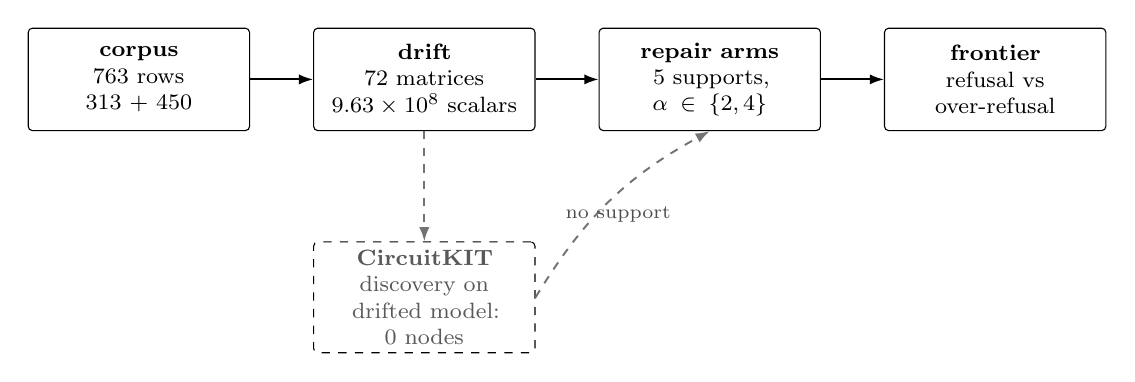
\begin{tikzpicture}[
    box/.style={draw, rounded corners=1.5pt, align=center, font=\footnotesize, inner sep=3pt,
                minimum height=13mm, text width=26mm},
    dead/.style={box, dashed, text=black!65},
    arr/.style={-{Latex[length=1.8mm,width=1.3mm]}, line width=0.7pt},
    darr/.style={arr, dashed, black!55},
    lab/.style={font=\scriptsize, align=center, text=black!70}]
  \node[box]  (c) {\textbf{corpus}\\763 rows\\313 + 450};
  \node[box, right=8mm of c]  (d) {\textbf{drift}\\72 matrices\\$9.63\times10^{8}$ scalars};
  \node[box, right=8mm of d]  (r) {\textbf{repair arms}\\5 supports,\\$\alpha\in\{2,4\}$};
  \node[box, right=8mm of r]  (f) {\textbf{frontier}\\refusal vs\\over-refusal};
  \node[dead, below=14mm of d] (k) {\textbf{CircuitKIT}\\discovery on\\drifted model: 0 nodes};
  \draw[arr]  (c) -- (d);
  \draw[arr]  (d) -- (r);
  \draw[arr]  (r) -- (f);
  \draw[darr] (d) -- (k);
  \draw[darr] (k.east) to[bend left=15] node[lab, pos=0.55, below=1pt] {no support} (r.south);
\end{tikzpicture}
\caption{The chain as executed. Solid arrows are executed stages. The dashed branch is the CircuitKIT
leg: it ran on the drifted model and returned an empty graph (\file{results/p6_circuit.json}), so no
circuit-derived support enters the repair arms or the frontier.}
\label{fig:pipeline}
\end{figure}

\section{The frontier}
\label{sec:frontier}

Table~\ref{tab:frontier} is the whole result. Rows are arms, ordered from the untouched model through the
drift to the repairs; the last three rows are the control of \S\ref{sec:control}. ``Support'' is the
fraction of weight columns the edit is allowed to touch. All values are read from
\file{evals/frontier.csv} (the file written by \file{experiments/p10_evals_bundle.py}), except the AUC
of the four arms the CSV does not contain, which is read from \file{results/p3b_sweep.json} and
\file{results/p3c_blind.json}; the caption marks that group. No number in this report is estimated.

\begin{table}[t]
\centering
\small
\setlength{\tabcolsep}{5pt}
\caption{Measured frontier. Refusal and over-refusal use the regex diagnostic; gsm8k is 120 items. AUC is
that of the drift direction as a linear separator. Every row comes from \file{evals/frontier.csv} except
the AUC of the four $\dagger$ rows, which comes from \file{results/p3b_sweep.json} and
\file{results/p3c_blind.json}.}
\label{tab:frontier}
\begin{tabular}{@{}lrrrrr@{}}
\toprule
\textbf{Arm} & \textbf{Support} & \textbf{Refusal} $\downarrow$ & \textbf{Over-refusal} $\downarrow$
& \textbf{gsm8k} & \textbf{AUC} \\
\midrule
base (aligned)                & ---     & 0.7583 & 0.0500 & 0.1167 & 0.9988 \\
drifted (abliterated)         & ---     & 0.2167 & 0.0000 & 0.1167 & 0.8306 \\
\midrule
global edit, $\alpha=4$       & 100\pct & 0.7417 & 0.5000 & 0.2167 & 0.789 \\
harm-ranked, 25\pct, $\alpha=4$ & 25\pct & 0.7083 & 0.4000 & 0.2750 & 0.821 \\
harm-ranked, 10\pct, $\alpha=4$ & 10\pct & 0.6083 & 0.3000 & 0.2667 & 0.790 \\
harm-ranked, 4\pct, $\alpha=4$  & 4\pct  & 0.5167 & 0.2250 & 0.2833 & 0.796 \\
harm-ranked, 2\pct, $\alpha=4$  & 2\pct  & 0.5083 & 0.2000 & 0.3000 & 0.795 \\
harm-ranked, 10\pct, $\alpha=2$ & 10\pct & 0.3667 & 0.0500 & 0.2000 & 0.814$^\dagger$ \\
\midrule
random support, 2\pct, $\alpha=4$  & 2\pct  & 0.2083 & 0.0250 & 0.108 & 0.824$^\dagger$ \\
random support, 10\pct, $\alpha=4$ & 10\pct & 0.2083 & 0.0000 & 0.125 & 0.861$^\dagger$ \\
amplitude-ranked, 10\pct, $\alpha=4$ & 10\pct & 0.5250 & 0.2250 & 0.275 & 0.780$^\dagger$ \\
\bottomrule
\end{tabular}
\end{table}

\begin{figure}[t]
\centering
\includegraphics[width=0.78\textwidth]{fig_frontier.pdf}
\caption{The same table as a plane. The line joins the $\alpha=4$ repair supports from 2\pct\ to the full
global edit; the star is the aligned model, the cross the drifted one, the open diamond the separate
$\alpha=2$ dose. Up and to the left is better. Figure generated by \file{report/fig_frontier.py} from
\file{evals/frontier.csv}.}
\label{fig:frontier}
\end{figure}

\textbf{The drift is real and large.} Refusal falls from 0.7583 to 0.2167 and over-refusal to exactly
zero; the direction's separability collapses from AUC 0.9988 to 0.8306. Capability, at gsm8k, does not move
at all (0.1167 to 0.1167). That is the signature of a deleted read-out rather than a damaged model, and it
is part one of the hypothesis confirmed.

\textbf{The global edit restores refusal but destroys discrimination.} At its full budget the global
rank-one repair recovers 97.0\% of the lost refusal (0.7417) --- and raises over-refusal from 0.0500 to
0.5000, ten times the aligned model's rate, on 20 of 40 benign prompts. In the plane of
Figure~\ref{fig:frontier} it is the extreme right-hand point: nearly all of the refusal, at a price the
aligned model never pays. Measured as refusal recovered per unit of over-refusal it is 1.48, the worst
arm on the board.

\textbf{Restriction buys the trade-off, but does not win the arm.} At 2\pct\ support --- 19{,}251{,}200
scalars, one fiftieth of the global patch --- refusal is 0.5083, i.e.\ 53.8\% of the gap recovered, for an
over-refusal of 0.2000: 2.54 units of refusal per unit of over-refusal, 1.7 times the global edit's rate.
The 4\pct\ arm lands within noise of it (0.5167 at 0.2250), so the curve has a plateau between 2\pct\ and
4\pct\ rather than a peak. This is the weaker form of part three: the restricted repair trades better per
unit of over-refusal and for a fiftieth of the edit, but no restricted arm reaches the base refusal rate,
and the global edit remains the highest-refusal arm overall.

\textbf{The cheap end is very cheap.} The 10\pct\ support at $\alpha=2$ gives 0.3667 refusal at an
over-refusal of 0.0500 --- exactly the aligned model's over-refusal --- for 27.6\% of the gap. It is the
point a deployment with a hard over-refusal budget would pick, and it is 7.3 units of refusal per unit of
over-refusal.

\textbf{AUC never comes back.} No arm, including the two inert random controls, leaves the 0.780--0.861
band, against 0.9988 for the aligned model. Repaired behaviour is recovered by amplifying a direction that
is a worse separator than the original one; the two inert controls with the \emph{highest} AUC (0.824 and
0.861) prove that AUC does not track behaviour. This is part two of the hypothesis: the cost is paid in
discrimination, not in capability, and over-refusal --- not AUC --- is the sensitive axis.

\textbf{gsm8k drifts upward, and that is not a capability gain.} Accuracy rises from 0.1167 on the drifted
model to 0.3000 at the 2\pct\ support. The model is at 0.1167 because abliteration destroyed its
chain-of-thought format, not its arithmetic; restoring a refusal direction restores some formatting, so
part of the gsm8k movement is format recovery. It is a direction, not a magnitude, and it is reported as a
diagnostic.

\section{The control}
\label{sec:control}

Two control supports separate ``which columns'' from ``how they were ranked''. At the same size and the
same $\alpha$, a random support of weight columns does nothing; a support ranked by write amplitude alone,
with no harm weighting, does most of the work.

\begin{table}[h]
\centering
\small
\caption{Control arms at $\alpha=4$. The drifted model is 0.2167; a random support is indistinguishable
from it at both sizes. Values from \file{results/p3c_blind.json}.}
\label{tab:control}
\begin{tabular}{@{}lrrr@{}}
\toprule
\textbf{Support selection} & \textbf{Support} & \textbf{Refusal} & \textbf{Over-refusal} \\
\midrule
random columns            & 2\pct  & 0.2083 & 0.0250 \\
random columns            & 10\pct & 0.2083 & 0.0000 \\
amplitude-ranked (no harm) & 10\pct & 0.5250 & 0.2250 \\
harm-ranked (main arm)     & 10\pct & 0.6083 & 0.3000 \\
\bottomrule
\end{tabular}
\end{table}

Random supports are inert: 0.2083 at 2\pct\ and 0.2083 at 10\pct, against 0.2167 for the untouched
drifted model. Neither recovers a single point of the gap, at either size. The choice of support is
therefore the whole effect, and it is not an artefact of editing a small number of weights.

Amplitude ranking alone, with no harm weighting, reaches 0.5250 at 10\pct\ --- 56.9\% of the gap, about
four-fifths of what the harm-weighted 10\pct\ arm achieves (0.6083, 72.3\%). So the harm-weighted ordering
is worth 8.3 points of refusal at that support, and the two are close: at matched 10\pct\ the harm-ranked
arm buys more refusal at a higher over-refusal (2.03 versus 2.33 units of refusal per unit of
over-refusal), and neither dominates. The honest reading is that harm weighting is an \emph{ordering} that
improves a support already selected by write amplitude; it is not the mechanism. The mechanism is that a
refusal direction lives in a small set of high-write columns, and any ordering that lands on them works.

The sharpest comparison in the whole study is between the harm-ranked 2\pct\ arm (0.5083 at 0.2000, 19.3M
scalars) and the amplitude-ranked 10\pct\ arm (0.5250 at 0.2250, 96.3M scalars). They differ by 1.7 points
of refusal and 2.5 points of over-refusal --- both well inside the sampling noise of 120 and 40 prompts ---
for a fivefold difference in edit size. On this measurement the two are indistinguishable behaviourally;
the difference that is not noise is the size of the patch.

\section{What did not work}
\label{sec:failed}

This section is deliberately not softened. Three of the five stages produced a usable result; the
circuit stage produced nothing and the audit stage produced one contested number; a reader needs the
second half more than the first.

\textbf{The circuit leg returned an empty graph.} \file{experiments/p6_circuit.py} ran CircuitKIT's
EAP-IG discovery at node level, 24 contrastive pairs, on the drifted model in TransformerLens, on an
A100-80GB in 64.8\,s. The drift was confirmed applied inside the same job (962{,}592{,}768 scalars,
$\cos(d,d') = 0.0035$). The result is
\file{results/p6_circuit.json}: \texttt{n\_nodes\_scored: 0}, \texttt{n\_circuitkit\_scores: 0}, an empty
layer histogram, \texttt{mass\_top40\_abs: 0.0}. Three friction points were found and recorded: Modal
requires \texttt{image.add\_local\_*} to be the last image step; CircuitKIT hard-imports third-party
packages at package-import time (\file{backends/acdc/types.py:6} imports \texttt{plotly}), so the
dependency has to be installed even though no plot is drawn; and contrastive token alignment discarded
every record --- the error line is \texttt{All 16 records were dropped during alignment
(strategy='filter')}, with \texttt{dropped\_misaligned: 24} --- which is why the run used
\texttt{align\_strategy="none"}. The consequence is stated plainly: \emph{there is no circuit result in
this submission}. H1 and H2 as pre-registered (a circuit-derived support beats a random one; circuit
localisation identifies the write columns) are untested, not refuted; the support was chosen by
harm-weighted write amplitude instead, and the negative result is that a discovery tool can run to
completion on a correct model and return nothing at all.

\textbf{One replicate never reported.} The third model in the replication set never produced a file. No
\texttt{water} result exists in \file{results/}, no \texttt{[done]} line appears in
\file{logs/p4_replicate.log}, and it is therefore not claimable and not in any table. Two of the three
replicates did land (\texttt{global} and \texttt{earth}, both reproducing the drift and the global repair).

\textbf{The judge panel was measured on two arms and disagreed with itself.} Automated ASR from the
four-judge panel exists for exactly two arms, because those were the only two in
\file{results/p3_support.json} when \file{experiments/p5_judge.py} ran. On the global arm the judges span
0.000 (Qwen3Guard) to 0.158 (Granite-Guardian); on the circuit/heads arm they span 0.000 to 0.400 --- a
40-point spread on the same completions, with a majority-of-three rate of 0.142. An earlier pilot on 12
prompts produced a 58-point spread across five judges (0.000 to 1.000) with pairwise agreement of
$\kappa \le 0.03$ (recorded in \file{_research/MEASUREMENT.md}), which is the reason the panel was never
promoted to a headline metric. Every ASR number
in this project is therefore either unmeasured or contested; the refusal regex is used throughout as a
\emph{diagnostic}, and this report never presents it as ASR.

\textbf{One arm was invalid and was withdrawn.} The first support experiment
(\file{results/p3_support.json}) costed a support in weighted-amplitude units against a scalar budget, so
every column passed the test and the ``circuit/harm'' arm edited all 470{,}016 columns --- a bit-identical
duplicate of the global edit, not a restricted one. It was superseded by \file{experiments/p3b_sweep.py}
and is not used anywhere above.

\textbf{The second model ran but its result was never retrieved.} \file{logs/p13_second_model.log}
records a completed run on the second model (refusal 0.525 at $\alpha=0$, over-refusal 0.050, gsm8k 0.242,
AUC 0.973, \texttt{[done]} with \texttt{wall\_s: 449.1}), but the JSON went to the Volume and was never
pulled into \file{results/}. It exists as a log line only and is not tabulated.

\section{Reproducibility}

Every number above is produced by one script into one file; Table~\ref{tab:repro} is that mapping, and the
commands follow it. Upstream repositories (\texttt{curatorkit}, \texttt{circuitkit}) are read-only and are
never vendored: they are added with \texttt{PYTHONPATH} and imported.


{\small
\begin{verbatim}
uv run python -m modal run experiments/p8_corpus.py
uv run python -m modal run experiments/p2_dose.py
uv run python -m modal run experiments/p3b_sweep.py          # alpha=4 sweep
uv run python -m modal run experiments/p3b_sweep.py          # alpha=2 arm
uv run python -m modal run experiments/p3c_blind.py
uv run python -m modal run experiments/p6_circuit.py
uv run python -m modal run experiments/p11_baseline_completions.py
uv run --with numpy python experiments/p10_evals_bundle.py
uv run --with matplotlib --with numpy python report/fig_frontier.py
\end{verbatim}
}

\file{experiments/p10_evals_bundle.py} reads the arm results and writes \file{evals/frontier.csv}; it is
the only thing standing between a JSON in \file{results/} and the figure in this report. The four patch
sets are published as \texttt{.npz} with a loader and a test suite, and the drifted checkpoint itself is
\emph{not} published --- see the last limitation.

\begin{table}[H]
\centering
\small
\caption{Script to result file; all scripts live in \file{experiments/}. Modal jobs are launched with the
local entrypoint, which is also the only writer of \file{results/*.json}.}
\label{tab:repro}
\begin{tabular}{@{}L{5.3cm}L{5.2cm}L{4.7cm}@{}}
\toprule
\textbf{Script} & \textbf{Produces} & \textbf{What it measures} \\
\midrule
\file{p8_corpus.py} & \file{1-curate/corpus/}\newline\file{corpus.jsonl}, \file{corpus_split.json} & curated corpus, frozen split, provenance \\
\file{p1_grid.py} & \file{results/p1_grid.json} & drift at reduced grid (40/20/64) \\
\file{p2_dose.py} & \file{results/p2_dose.json} & dose--response over $\alpha\in\{0,1,2,4,8\}$ \\
\file{patching.py} & \file{artifacts/*.npz} & the operator: direction, amplification, support \\
\file{p4_replicate.py} & \file{results/p4_replicate_*.json} & replication on two further models \\
\file{p3b_sweep.py} & \file{results/p3b_sweep.json} & five supports $\times$ $\alpha$; the frontier rows \\
\file{p3c_blind.py} & \file{results/p3c_blind.json} & random and amplitude-ranked controls \\
\file{p5_judge.py} & \file{results/p5_judge.json} & four-judge ASR, two arms only \\
\file{p6_circuit.py} & \file{results/p6_circuit.json} & CircuitKIT discovery (0 nodes scored) \\
\file{p11_baseline_completions.py} & \file{results/p11_baseline.json} & base and drifted baselines \\
\file{p10_evals_bundle.py} & \file{evals/frontier.csv} & the frontier file used by \S\ref{sec:frontier} \\
\bottomrule
\end{tabular}
\end{table}
\section{Limitations}

\begin{itemize}[leftmargin=1.2em,itemsep=2pt,topsep=2pt]
\item \textbf{Small evaluation sets.} Refusal is measured on 120 prompts and over-refusal on 40. One
prompt on the benign axis is 2.5 points, so differences of 2--3 points between arms (for example the
2\pct\ versus 4\pct\ repair) are inside the noise. Only differences of five points or more should be read
as findings.
\item \textbf{One drift seed, one layer, one direction.} The direction is fitted at layer 15 from 16+16
prompts and everything downstream inherits that choice. Nothing here establishes that another layer, or
another seed, yields the same frontier.
\item \textbf{The refusal metric is a regex diagnostic, not ASR.} It counts refusal markers; it cannot tell
a refusal from a broken generation. The $\alpha=8$ arm proves the failure mode: the regex reads 0.000 for
a model that has collapsed into repetition, which is the opposite of safe.
\item \textbf{The direction is English-only.} Prompts, the fitted direction and the evaluation set are
English. The multilingual machinery ran (59 languages merged) but no per-language result file exists, so
the cross-lingual hypothesis is measured-but-unreported here.
\item \textbf{No drifted checkpoint is published.} Under LSAL \S2 and \S4 the research licence permits
research use only, forbids product hosting, and forbids publishing or deploying a drifted checkpoint.
Only parameters are published --- the \texttt{.npz} patch plus a loader --- never a merged model.
\item \textbf{The circuit claim is absent.} Discovery returned zero scored nodes, so H1 and H2 remain
untested and no statement about circuits should be read into this report.
\end{itemize}

\end{document}
